% -*- mode: noweb; noweb-default-code-mode: R-mode; -*-
\documentclass[11pt]{article}
%% Set my margins
\setlength{\oddsidemargin}{0.0truein}
\setlength{\evensidemargin}{0.0truein}
\setlength{\textwidth}{6.5truein}
\setlength{\topmargin}{0.0truein}
\setlength{\textheight}{9.0truein}
\setlength{\headsep}{0.0truein}
\setlength{\headheight}{0.0truein}
\setlength{\topskip}{0pt}
%% End of margins

%%\pagestyle{myheadings}
%%\markboth{$Date$\hfil$Revision$}{\thepage}

\usepackage[pdftex,
bookmarks,
bookmarksopen,
pdfauthor={Zequn Sun, Wei Wei and Dongjun Chung},
pdftitle={INGRID Vignette}]
{hyperref}

% \usepackage{fullpage}
% \usepackage{pdflscape}

\title{An Introduction to the `\texttt{INGRID}' Package, Version 1.0}
\author{Zequn Sun,Wei Wei and Dongjun Chung\\
Department of Public Health Sciences, Medical University of South Carolina (MUSC),\\
  Charleston, SC, 29425.}


\date{\today}



\usepackage{Sweave}
\begin{document}
\Sconcordance{concordance:INGRID-example.tex:E:/Dr.Chung/2/INGRID/vignettes/INGRID-example.Rnw:%
1 36 1 1 0 22 1 1 4 1 2 4 0 1 2 11 1 1 2 1 0 1 1 10 0 1 1 5 0 1 1 5 0 1 %
1 12 0 1 2 4 1 1 2 1 0 1 1 34 0 1 2 5 1 1 2 1 0 1 1 10 0 1 2 7 1 1 2 4 %
0 1 3 11 0 1 2 2 1 1 2 9 0 1 2 13 1 1 2 1 0 1 1 16 0 1 2 2 1 1 2 13 0 1 %
2 2 1 1 2 4 0 1 2 5 1 2 2 6 1 1 2 4 0 1 2 5 1 1 2 30 0 1 2 4 1 1 2 4 0 %
1 2 4 1 2 2 7 1 1 2 4 0 1 2 3 1 2 2 14 1}

%\VignetteIndexEntry{INGRID}
%\VignetteKeywords{INGRID}
%\VignettePackage{INGRID}
%\VignetteEncoding{UTF-8}
\maketitle

\section{Overview}

This vignette provides basic information about the
\texttt{INGRID} package for the pathway-guided identification of cancer subtypes \cite{INGRID}. The proposed approach improves identification of molecularly-defined subgroups of cancer patients by utilizing information from pathway databases in the following four aspects.

(1) Integration of genomic data at the pathway-level improves robustness and stability in identification of cancer subgroups and driver molecular features;

(2) Summarizing multiple genes and genomic platforms at the pathway-level can potentially improve statistical power to identify important driver pathways because moderate signals in multiple genes can be aggregated;

(3) In \texttt{INGRID}, we consider the ``cooperation'' or ``interaction'' between pathways, instead assuming that each pathway operates independently during the cancer progression, which may be unrealistic;

(4) \texttt{INGRID} allows simultaneous inference in multiple biological layers (pathway clusters, pathways, and genes) within a statistically rigorous and unified framework without any additional laborious downstream analysis.

The package can be loaded with the command:


\begin{Schunk}
\begin{Sinput}
R> library("INGRID")
\end{Sinput}
\end{Schunk}

\section{Input Data}

The package requires that the response consist of 4 components:
(1) gene expression z-scores in the form of a either data frame or matrix;
(2) survival time and censoring indicator in the form of vectors;
(3) pathway information in the form of a list, where each element is a vector of the names of gene belonging to the pathway.

In this vignette, a small subset of the Cancer Genome Atlas (TCGA) data is used to illustrate the `\texttt{INGRID}' package. Specifically, we consider z-scores for the mRNA expression data of 389 genes for 50 randomly selected high-grade serous ovarian cancer patients, along with their survival times and censoring statuses. This dataset is included as an example data `\texttt{TCGA}' in the `\texttt{INGRID}' package. This TCGA data was originally downloaded from the cBio Portal (http://www.cbioportal.org/) using the R package `\texttt{cgdsr}' and here we consider z-scores for the mRNA expression data. The `\texttt{TCGA}' is a list object with four elements, including the `\texttt{geneexpr}' data frame of z-scores for the mRNA expression, the `\texttt{t}' vector of the survival time, the `\texttt{d}' vector of the censoring status indicator, and the `\texttt{pathList}' list of the pathway information. The `\texttt{pathList}' has four elements, each of which contains names of genes belonging to each pathway.

This dataset can be loaded as follows:

\begin{Schunk}
\begin{Sinput}
R> data(TCGA)
R> TCGA$geneexpr[1:5,1:5]
\end{Sinput}
\begin{Soutput}
        ACLY        ACO1       ACO2         CS       DLAT
1 -2.2410125 -0.48445531 -1.6346455  0.1378804 -3.5310321
2 -2.1301362  0.82116427 -0.9533701  0.6213512  0.6689948
3 -2.9122727 -0.08790649 -1.0975096 -0.2454025 -0.9433900
4 -1.1721514 -0.24249825 -0.7212639  0.1842386 -0.6188785
5  0.5383438  0.98012739 -0.7396043 -0.0699680  1.9573767
\end{Soutput}
\begin{Sinput}
R> TCGA$t[1:5]
\end{Sinput}
\begin{Soutput}
[1] 43.89 40.97 49.12  2.00 46.59
\end{Soutput}
\begin{Sinput}
R> TCGA$d[1:5]
\end{Sinput}
\begin{Soutput}
[1] 1 1 0 1 0
\end{Soutput}
\begin{Sinput}
R> TCGA$pathList[1]
\end{Sinput}
\begin{Soutput}
$KEGG_CITRATE_CYCLE_TCA_CYCLE
 [1] "IDH3B"     "DLST"      "PCK2"      "CS"        "PDHB"      "PCK1"     
 [7] "PDHA1"     "LOC642502" "PDHA2"     "LOC283398" "FH"        "SDHD"     
[13] "OGDH"      "SDHB"      "IDH3A"     "SDHC"      "IDH2"      "IDH1"     
[19] "ACO1"      "ACLY"      "MDH2"      "DLD"       "MDH1"      "DLAT"     
[25] "OGDHL"     "PC"        "SDHA"      "SUCLG1"    "SUCLA2"    "SUCLG2"   
[31] "IDH3G"     "ACO2"     
\end{Soutput}
\end{Schunk}

\section{Gene Regrouping}
Gene Grouping step is to redefine the gene set membership of common genes. First, the gene remains to be as a member if it is a core member of the pathway.  A gene is defined as a “core
member” of a pathway if it belongs to only that pathway.  Second, if the gene is not a core member of any among the pathways (i.e., it maps to more than one pathways), then this gene is re-assigned to one of the gene sets based on the k-medoids algorithm minimizing the binary distance between genes within cluster distance.

\begin{Schunk}
\begin{Sinput}
R> geneRegroup.results <- geneRegroup(TCGA$pathList)
R> geneRegroup.results
\end{Sinput}
\begin{Soutput}
Summary: Gene-Regrouping results (class: RegroupGene)
--------------------------------------------------
Gene sets before gene regrouping
List of 4
 $ KEGG_CITRATE_CYCLE_TCA_CYCLE   : chr [1:32] "IDH3B" "DLST" "PCK2" "CS" ...
 $ KEGG_MAPK_SIGNALING_PATHWAY    : chr [1:267] "JUN" "MEF2C" "ELK4" "ELK1" ...
 $ KEGG_TGF_BETA_SIGNALING_PATHWAY: chr [1:86] "TFDP1" "NOG" "TNF" "GDF7" ...
 $ KEGG_THYROID_CANCER            : chr [1:29] "PAX8" "HRAS" "CCDC6" "TFG" ...
--------------------------------------------------
Gene sets after gene regrouping
List of 6
 $ NTRK1                          : chr [1:8] "NRAS" "KRAS" "MAP2K2" "MAP2K1" ...
 $ TGFB2                          : chr [1:9] "MYC" "TGFB2" "TGFB1" "TGFBR2" ...
 $ KEGG_CITRATE_CYCLE_TCA_CYCLE   : chr [1:32] "IDH3B" "DLST" "PCK2" "CS" ...
 $ KEGG_MAPK_SIGNALING_PATHWAY    : chr [1:250] "JUN" "MEF2C" "ELK4" "ELK1" ...
 $ KEGG_TGF_BETA_SIGNALING_PATHWAY: chr [1:77] "TFDP1" "NOG" "GDF7" "INHBB" ...
 $ KEGG_THYROID_CANCER            : chr [1:18] "PAX8" "CCDC6" "TFG" "NCOA4" ...
--------------------------------------------------
Pathway names before gene regrouping
                             Pathway Name
pathway_1    KEGG_CITRATE_CYCLE_TCA_CYCLE
pathway_2     KEGG_MAPK_SIGNALING_PATHWAY
pathway_3 KEGG_TGF_BETA_SIGNALING_PATHWAY
pathway_4             KEGG_THYROID_CANCER
--------------------------------------------------
Number of genes in new gene set that are from the old pathway
      pathway_1 pathway_2 pathway_3 pathway_4
NTRK1         0         8         0         8
TGFB2         0         9         9         3
\end{Soutput}
\end{Schunk}
The table above shows the number of genes of a new gene set that is from the original pathways. For instance, the new gene set "NTRK1" has 0 gene from "pathway_1", which is "KEGG_CITRATE_CYCLE_TCA_CYCLE", 8 genes from "pathway_2", which is "KEGG_MAPK_SIGNALING_PATHWAY", and so on.

\section{Pre-filtering}

To refine the candidate set of genes, we first conduct a supervised pre-filtering by fitting a Cox regression model of the mRNA expression measure of each gene on the patient survival. Only the gene expressions associated with patient survival at p-values smaller than a pre-specified cut-off are included in the subsequent analysis. By default, p = 0.5 is used as cut-off point.

\begin{Schunk}
\begin{Sinput}
R> prefilter.results <- prefilter( data=TCGA$geneexpr, time=TCGA$t, status=TCGA$d, plist=geneRegroup.results@gset )
R> prefilter.results
\end{Sinput}
\begin{Soutput}
Summary: Pre-filtering results (class: Prefiltered)
--------------------------------------------------
Number of genes before prefiltering: 389
Number of genes after prefiltering: 213
--------------------------------------------------
\end{Soutput}
\end{Schunk}


\section{Gene Selection}

In order to select key genes associated with patient survivals and effectively summarize them by taking into account correlation among them, we fit a sparse partial least squares (SPLS) Cox regression model \cite{SPLS} of patient survivals on gene expression measurements for each pathway.

Using the object `\texttt{prefilter.results}', gene-level analysis result can be generated with `\texttt{selectGene}' function as follows.

\begin{Schunk}
\begin{Sinput}
R> gene.results <- selectGene(prefilter.results)
\end{Sinput}
\end{Schunk}
\begin{Schunk}
\begin{Sinput}
R> gene.results
\end{Sinput}
\begin{Soutput}
Summary: Gene-level analysis results (class: FitGene)
--------------------------------------------------
Number of prefiltered genes: 213
Number of selected genes: 130
--------------------------------------------------
\end{Soutput}
\end{Schunk}

The list of the SPLS regression coefficients of cancer-related genes can be generated using the function \texttt{coef()}.

\begin{Schunk}
\begin{Sinput}
R> head(coef(gene.results)[[1]])
\end{Sinput}
\begin{Soutput}
  colnames.xx..spls.mod.A.    betahat
1                     NRAS -0.4465544
2                     TP53 -0.4754562
\end{Soutput}
\end{Schunk}

The function `\texttt{selectGene}' has two main tuning parameters: `\texttt{eta}' represents the sparsity tuning parameter and `\texttt{K}' is the number of hidden (latent) components. Parameters can be chosen by ($v$-fold) cross-validation. Users can search the range for these parameters and the cross-validation procedure searches within these ranges. Note that `\texttt{eta}' should have a value between 0 and 1 while `\texttt{K}' is integer-valued and can range between
1 and $ min \left\{ p, (v-1) n / v \right\} $, where $p$ is the number of genes and $n$ is the sample size. For example, if 10-fold cross-validation is used (default), `\texttt{K}' should be smaller than $ min \left\{ p, 0.9 n \right\} $. For the TCGA data, we set the number of folds as 5, `\texttt{K}' as 5, and search  the optimal `\texttt{eta}' in the range between 0.1 and 0.9.

\section{Pathway Selection}

Next, in order to identify a parsimonious set of pathways associated with patient survivals, we fit a LASSO-penalized Cox regression \cite{LASSO} on latent components derived from all the pathways.
Specifically, a pathway is selected if at least one of its latent components has non-zero LASSO coefficient estimate.

This approach has the following two strengths:
First, the latent components generated from the SPLS step preserve pathway structure and also reflect correlation among genes and their association with survival outcomes. Second, this approach can potentially improve the stability of estimation in the subsequent analysis.

Using the `\texttt{gene.results}', pathway-level analysis result can be generated with `\texttt{selectPath}' function.

\begin{Schunk}
\begin{Sinput}
R> path.results <- selectPath(gene.results)
R> path.results
\end{Sinput}
\begin{Soutput}
Summary: Pathway-level analysis results (class: FitPath)
--------------------------------------------------
Number of all pathways: 6
Number of selected pathways: 4

List of selected pathways:
	NTRK1:
	KEGG_CITRATE_CYCLE_TCA_CYCLE:
	KEGG_MAPK_SIGNALING_PATHWAY:
	KEGG_TGF_BETA_SIGNALING_PATHWAY:
--------------------------------------------------
\end{Soutput}
\end{Schunk}

LASSO regression coefficients of cancer-related pathways can be generated using the function \texttt{coef()}.

\begin{Schunk}
\begin{Sinput}
R> head(coef(path.results))
\end{Sinput}
\begin{Soutput}
              rep.pathways..cols. path.beta
1                           NTRK1 0.2051799
2                           NTRK1 0.0000000
3                           TGFB2 0.0000000
4    KEGG_CITRATE_CYCLE_TCA_CYCLE 0.2169771
5     KEGG_MAPK_SIGNALING_PATHWAY 0.1828202
6 KEGG_TGF_BETA_SIGNALING_PATHWAY 0.0918629
\end{Soutput}
\end{Schunk}

Hazard ratio plot associated with each latent component in the selected pathways can be generated using the function \texttt{plot()} with the argument \texttt{type="{}HR"{}}.

\begin{Schunk}
\begin{Sinput}
R> plot(path.results, type="HR")
\end{Sinput}
\end{Schunk}

Figure 1 shows the hazard ratio (HR) associated with each latent component in the pathways selected by the \texttt{INGRID}.
Based on the TCGA data, pathways with the largest effect on survival (HR $\geq 1.15$) are \texttt{KEGG\_CITRATE\_CYCLE\_TCA\_CYCLE} and \texttt{KEGG\_TGF\_BETA\_SIGNALING\_PATHWAY} pathways.

\begin{figure}[tbh]
\begin{center}
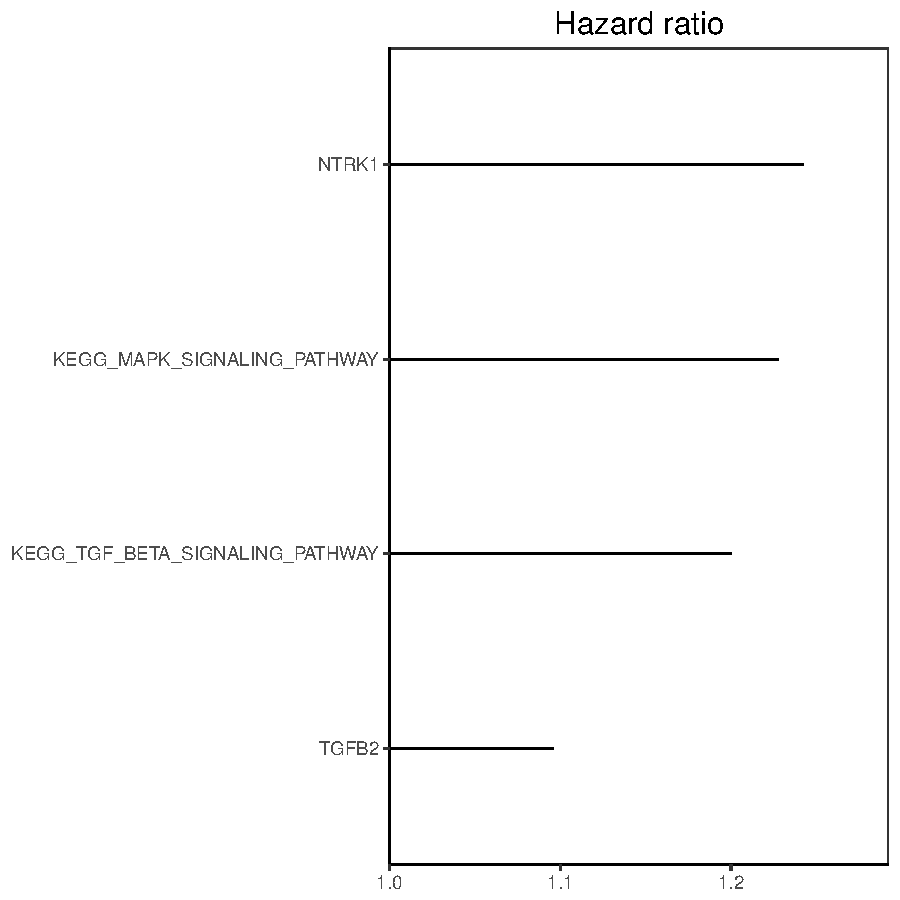
\includegraphics{INGRID-example-plot1}
\caption{Hazard ratio (HR) associated with each latent component in selected pathways.}
\end{center}
\end{figure}

\section{Risk Group Prediction}
Risk group predictions can be made using the function \texttt{predict()}

\begin{Schunk}
\begin{Sinput}
R> predicted <- predict(path.results)
\end{Sinput}
\end{Schunk}

The function `\texttt{predict}' returns a list with the following three elements:
(1) \texttt{risk.index}: number of pathways with elevated activity for each patient;
(2) \texttt{riskcat}: risk group prediction for each patient;
(3) \texttt{cuts}: cut off to determine low, intermediate and high risk groups.

\begin{Schunk}
\begin{Sinput}
R> predicted
\end{Sinput}
\begin{Soutput}
$risk.index
 [1] 2 4 1 4 1 3 4 0 0 1 4 0 2 2 2 3 0 1 2 1 1 1 0 1 3 3 2 0 1 1 2 1 1 0 1 1 0 2
[39] 3 2 1 2 2 3 4 4 2 3 4 3

$riskcat
 [1] "med"  "high" "low"  "high" "low"  "high" "high" "low"  "low"  "low" 
[11] "high" "low"  "med"  "med"  "med"  "high" "low"  "low"  "med"  "low" 
[21] "low"  "low"  "low"  "low"  "high" "high" "med"  "low"  "low"  "low" 
[31] "med"  "low"  "low"  "low"  "low"  "low"  "low"  "med"  "high" "med" 
[41] "low"  "med"  "med"  "high" "high" "high" "med"  "high" "high" "high"

$cuts
[1] 1 3

$time
 [1]  43.89  40.97  49.12   2.00  46.59  18.50  11.86  65.44  63.01  48.72
[11]  21.55  63.93  49.25  32.49  44.29  33.64  76.48  71.42  56.51  19.97
[21]  38.34 118.99  84.14  57.69  35.51   9.95  38.41  89.26  41.56  57.53
[31]  30.46   6.11  35.12 112.29  71.06  63.05  39.72  12.45  25.89  81.80
[41]  18.46  34.17  32.85  14.65   6.67  35.38  19.97  20.89   6.21  24.57

$status
 [1] 1 1 0 1 0 1 1 0 0 1 1 1 1 0 1 1 0 0 1 1 1 1 1 1 1 1 1 1 1 0 0 0 1 0 0 0 0 0
[39] 1 1 1 1 1 1 1 1 1 1 1 1
\end{Soutput}
\end{Schunk}

\section{Survival Curve}

The predictive performance of \texttt{INGRID} method can be presented by Kaplan-Meier curves. Kaplan-Meier curves of predicted patient subgroups can be generated with \texttt{plot()} function with argument \texttt{type="{}KM"{}}.

\begin{Schunk}
\begin{Sinput}
R> plot(path.results, type="KM")
\end{Sinput}
\end{Schunk}

Figure 2 shows the Kaplan-Meier curves of predicted patient subgroups and indicates that the \texttt{INGRID} approach successfully separates out high, intermediate and low risk groups.

\begin{figure}[tbh]
\begin{center}
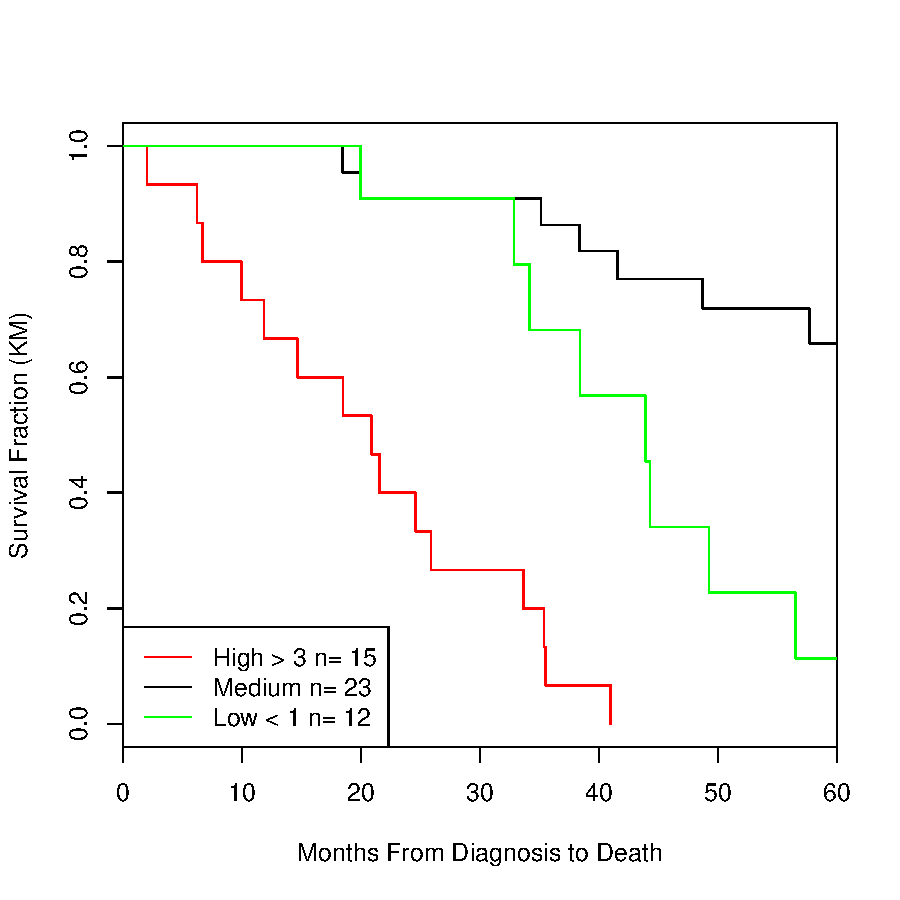
\includegraphics{INGRID-example-plot}
\caption{The observed survival curves for patient subgroups.}
\end{center}
\end{figure}

\section{Survival ROC}

The predictive performance of \texttt{INGRID} method can be further evaluated based on area under the time dependent receiver operating curve (ROC).
ROC plot can be generated using \texttt{plot()} function with argument \texttt{type="{}ROC"{}}.
\begin{Schunk}
\begin{Sinput}
R> plot(path.results, type="ROC")
\end{Sinput}
\end{Schunk}


\begin{figure}[tbh]
\begin{center}
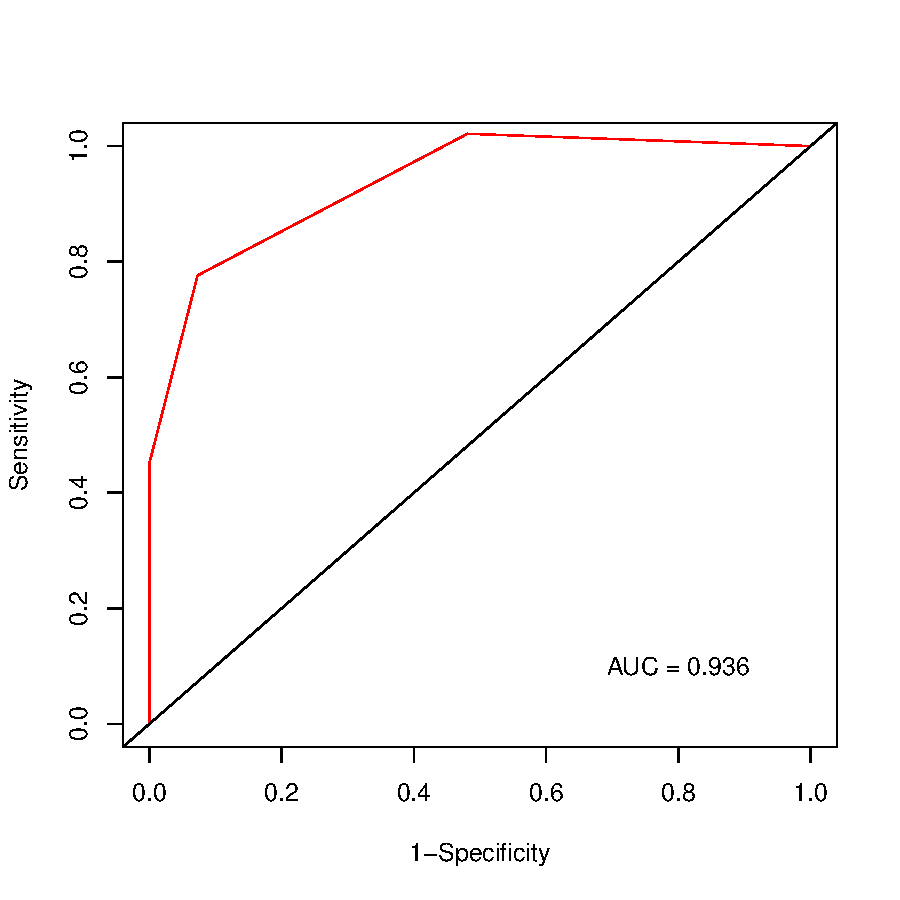
\includegraphics{INGRID-example-plot3}
\caption{Time dependent receiver operating curve}
\end{center}
\end{figure}

Figure 3 shows the ROC curves for survival, and for the TCGA data, the area under curve (AUC) associated with the \texttt{INGRID} approach was 0.936.

\begin{thebibliography}{99}
\bibitem{INGRID} Wei W., Zequn S., Willian S., Zhenning Y., Andrew L., Gary H., Linda K., Dongjun C. (2017), ``INGRID: Semi-supervised Identification of Cancer Subgroups using Survival Outcomes and Overlapping Grouping Information''. (submitted).
\bibitem{TCGA} Cancer Genome Atlas Research Network (2011), ``Integrated genomic analyses of ovarian carcinoma''. Nature, 474(7353), 609-615.
\bibitem{SPLS} Bastien, P., Bertrand, F., Meyer, N., Maumy-Bertrand, M. (2014), `` Deviance residuals-based sparse PLS and sparse kernel PLS regression for censored data''. Bioinformatics, 31(3), 397-404.
\bibitem{LASSO} Tibshirani, R. (1997), ``The lasso method for variable selection in the cox model''. Statistics in Medicine, 16(4), 385-395.

\end{thebibliography}

\end{document}
